\documentclass[mathserif,usenames,dvipsnames]{beamer}

\usepackage{multicol}
\usepackage{beamerthemeshadow}
\usepackage{graphicx}
\usepackage{graphics}
\usepackage{pgf}
\usepackage{tikz, ifthen}
%\usepackage{scalefnt}
\usepgfmodule{shapes}
\usepgfmodule{plot}
\usetikzlibrary{shapes,arrows,shadows,fit}
\usepackage{hyperref}   % Hyperlink references and URLs
\usetikzlibrary{arrows,automata,petri,positioning}
\usepackage[latin1]{inputenc}

%% Hack so 'backup' slides aren't reflected in total slide count
\newcommand{\backupbegin}{
       \newcounter{framenumberappendix}
          \setcounter{framenumberappendix}{\value{framenumber}}
}
\newcommand{\backupend}{
       \addtocounter{framenumberappendix}{-\value{framenumber}}
          \addtocounter{framenumber}{\value{framenumberappendix}} 
}

\title[AHOY: Slide \insertframenumber/\inserttotalframenumber]{AHOY: A Distributed, Event-Based Simulation Environment for Networked Multi-Agent Systems}

\subtitle{Final Presentation}

\author[Clark, Ingram, Kolakowska, \& Rosenfeld]{ 
Frank~Clark\inst{1}, Dustin~Ingram\inst{1}, Maria~Kolakowska\inst{1}, Aaron~Rosenfeld\inst{1}, William~Regli\inst{1}}

\institute{
    \inst{1}%
    Drexel University Department of Computer Science, Philadelphia PA
}

\date{\today}

\begin{document}

\frame{\titlepage} 

\frame
{
    \frametitle{Outline}
    \tableofcontents
}

\frame
{   
    \frametitle{Abstract}
    \textit{Abstract:} AHOY is a distributed, event-based simulation environment designed to test networked multi-agent systems.
}

\section{Introduction}
\frame
{
\begin{center}
    \begin{tabular}{c c}
    
\includegraphics[scale=.2]{drexel.png} & 
\includegraphics[scale=.6]{nrl.png} \\
    
\includegraphics[scale=.25]{acin.png} & 
\includegraphics[scale=.25]{cvut.png} \\
    \end{tabular}
\end{center}
}
\frame
{
    \begin{center}
        
\includegraphics[scale=.4]{../common/logo.pdf}
    \end{center}
}
\frame
{
    \begin{center}
        \includegraphics[scale=.5]{../mindmap/mindmap1.pdf}
    \end{center}
}
\frame
{
    \begin{center}
        \includegraphics[scale=.75]{../mindmap/mindmap2.pdf}
    \end{center}
}
\frame
{
    \begin{center}
        \includegraphics[scale=.55]{../mindmap/mindmap3.pdf}
    \end{center}
}

\frame
{
    \frametitle{Overview of AHOY}
    \begin{itemize}
	\item Event-based simulation environment
	\item Used to compare combinations of software agents, network configurations, and sensor data in real-world environments
	\item Physically Distributed Simulation
	\item ``Programming'' Interface:
	\begin{itemize}
	    \item Agent Software
	    \item Network Topologies
	    \item Sensor Functions
	    \item World Objects
	\end{itemize}
	\item Rapid scenario creation
	\item Bridges network emulators and agent simulators
    \end{itemize}
}

\subsection{Network Simulators}
\frame
{
    \frametitle{Background on Network Simulators}
    \begin{itemize}
        \item Application and protocol testing without physical hardware
        \item Mimic the properties of a physical network
        \item Network compents are virtualized (``nodes'') 
        \item Allow multiple virtual nodes to run on one physical machine
        \item Scale well, easy to re-configure
        \item Cost \& time effective
    \end{itemize}
}

\subsection{Agent Frameworks}
\frame
{
    \frametitle{Background on Agents \& Agent Frameworks}
    \begin{block}{Definition}
    An \emph{intelligent agent} is software which observes and acts upon an environment and directs its activity towards achieving goals (Russell, Norvig).
    \end{block}

    \textbf{Agent Simulators}
    \begin{itemize}
        \item Used to test agent algorithms within virtual worlds
        \item Rules define actions to be taken based on beliefs
        \item Agent rule-sets react to sensory information in the world
        \item Allows for large-scale simulation unfeasible in the real-world
    \end{itemize}
}

\subsection{Issues with Existing Tools}
\frame
{
    \frametitle{Existing tools}
    \textbf{Current Network Simulators}
    \begin{itemize}
        \item Designed for testing networks \& protocols, not agents 
        \item Scenarios are pre-scripted
        \item Poor event support
        \item Inability to vary settings across batch scenario executions
        \item Data collection non-existent or not directly supported
    \end{itemize}
    \textbf{Current Agent Frameworks}
    \begin{itemize}
        \item Communications modeled only at the application layer
        \item Lack of rich lower-level protocols, or
        \item Require physical hardware for networking
    \end{itemize}
}

\section{Motivation}
\frame
{
    \frametitle{Motivational Background}
    \textbf{Current Network Simulators}
    \begin{itemize}
	\item Existing simulation engines not designed for testing agents but for testing the network \& protocols (NS2/3)
	\item Pre-scripted scenarios (CORE) or poor event support (EMANE)
	\item Lack of templated agents
	\item Inability to batch process many executions of scenarios with varying settings
	\item Data collection non-existent or not supported
    \end{itemize}
    \textbf{Current Agent Frameworks}
    \begin{itemize}
	\item Communications modeled only at the application layer (send/recv)
	\item Lack of rich lower-level protocols
	\item Alternative approaches (Player project) require physical hardware for networking
    \end{itemize}
}

\subsection{CORE}
\frame
{
    \frametitle{Motivational Background - CORE}
    \begin{itemize}
	\item CORE is a network emulator which allows software to be run inside virtual machines with full network stacks
	\item Uses Linux network namespaes (netns), a lightweight container-based virtualization similar to FreeBSD ``jail''
	\item Basic implementation of PHY and MAC layer protocols including 802.11 and Ethernet
	\item Extremely easy to create scenarios; drag and drop interface
	\item Currently being developed by Boeing, based on the open source Integrated Multiprotocol Emulator/Simulator (IMUNES) project developed by the University of Zagreb
    \end{itemize}
}

\frame
{
    \frametitle{Motivational Background - CORE}
    \begin{center}
        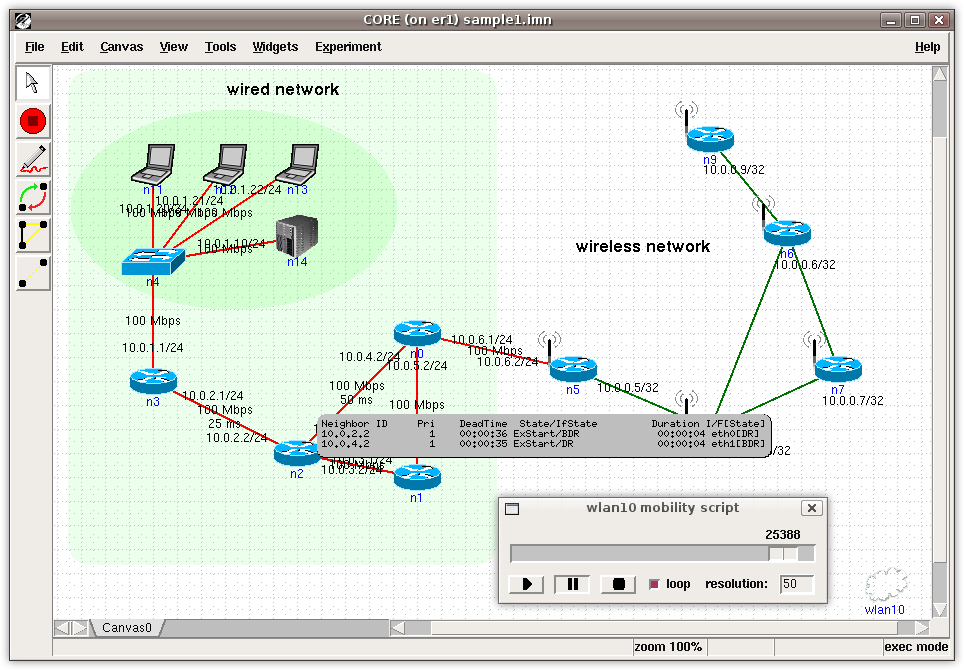
\includegraphics[scale=.25]{core-screenshot.png}
    \end{center}
}

\subsection{EMANE}
\frame
{
    \frametitle{Motivational Background - EMANE}
    \begin{itemize}
	\item EMANE is an Extendable Mobile Ad-hoc Network Emulator
	\item Allows heterogeneous network emulation using a plugable MAC and PHY layer architecture
	\item Pre-scripted scenarios publich timed events to a common event channel
	\item 1-to-1 virtual-to-physical node mapping (without additional virtualization)
	\item No GUI or integrated visualization component
	\item EMANE is an Open Source project developed by CenGen, Inc., Columbia, Maryland and released under the BSD license
    \end{itemize}
}

\subsection{NS3}
\frame
{
    \frametitle{Motivational Background - NS3}
    \begin{itemize}
	\item Well known network simulator with proven accurate network stack characteristics
	\item Command line based
	\item Allows developers to write applications and define scenarios in C/C++
	\item Simulated -- results in slower-than-realtime experiments
	\item Applications must be written from scratch; no notion of agents or modularity
    \end{itemize}
}

\section{Implementation}
\subsection{Goals}
\frame
{
    \frametitle{Implementation Goals}
    \textbf{Bridge network simulators and agent simulators}
    \begin{itemize}
        \item Entirely event-driven
        \item Real-time
        \item Allow for human-in-the-loop interaction with agents
        \item Enable scenarios and network topologies to be easily defined
        \item Make writing custom agents extremely simple
        \item Visualization flexibility
        \item Physically distributed simulation
        \item Simple data collection
    \end{itemize}
}

\subsection{Overview}
\frame
{
    \frametitle{Event-Based Simulation}
    \textbf{Events allow Agents to react in real-time}
    \begin{itemize}
        \item Every action or change in the simulation is an event
        \item All events are passed over the event channel
        \item Event channel is available to all virtual nodes, agents
        \item Physical nodes as well, including visualizers
        \item New events can be inserted in real-time (human-in-the-loop)
    \end{itemize}
}

\frame
{
    \frametitle{Scaled Distribution}
    \textbf{Virtual Nodes}
    \begin{itemize}
	\item Very simple to distribute as all events are broadcast over a common event channel
	\item Future prototype will include method of starting agents on multiple physical machines
	\item Synchronization of simulation-time across physical machines may prove difficult, especially with integration of NS3; possible issues with human-in-the-loop
    \end{itemize}
    \textbf{Simulation Engine}
    \begin{itemize}
	\item Simulation engine may become a bottleneck as all ``filter \& forward'' (e.g. messaging) type events must flow through it
	\item Distribution of simulation engine is a future goal 
    \end{itemize}
}

\frame
{
    \frametitle{Decoupled Visualization}
    \textbf{Visualizing the Simulation}
    \begin{itemize}
        \item Monitoring the event channel produces raw event data
        \item Occurs simultaneously with the execution of an experiment
        \item Visualizers interpret events, produce their own representation 
        \item Completely separated from the simulator
    \end{itemize}
}

\frame
{
    \frametitle{Scenario Setup \& Creation}
    \textbf{Using a ``Programming'' Interface}
    \begin{itemize}
        \item Each of the following are defined purely in Python:
        \begin{itemize}
            \item Agent Behaviors 
            \item Network Topologies
            \item Sensor Functionality
            \item World Objects \& Behaviors
        \end{itemize}
        \item These definitions are then interpreted by the simulator
        \item Sets up the experiment \& defines the scenario
    \end{itemize}

}

\frame
{
    \frametitle{CS485/511: Predator/Prey Assignment}
    \begin{center}
        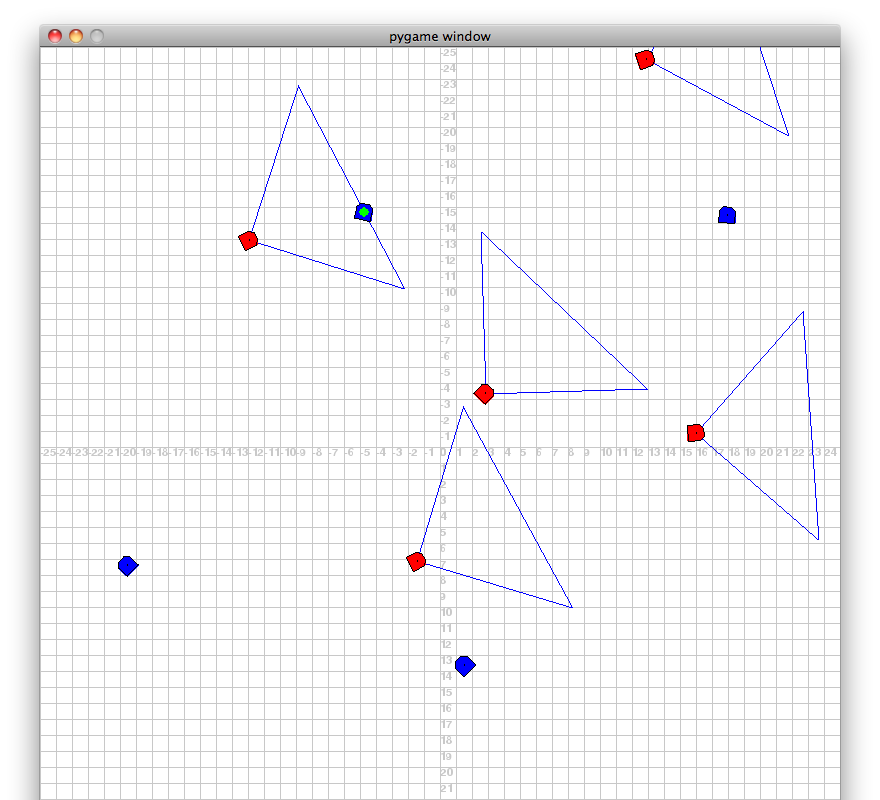
\includegraphics[scale=.23]{pp.png}
    \end{center}
}

\frame
{
    \frametitle{Contact \& Links}
    \begin{center}
	Dustin S. Ingram - \texttt{dustin@cs.drexel.edu} \\
	Aaron M. Rosenfeld - \texttt{ar374@cs.drexel.edu} \\
	Maria J. Kolakowska - \texttt{mjk75@cs.drexel.edu} \\
	Frank J. Clark - \texttt{fjc28@cs.drexel.edu} \\
	William C. Regli - \texttt{regli@cs.drexel.edu} \\
    \end{center}

    \textbf{AHOY:} http://ahoy.googlecode.com/ \\
    \textbf{CORE:} http://cs.itd.nrl.navy.mil/work/core \\
    \textbf{EMANE:} http://cs.itd.nrl.navy.mil/work/emane \\
    \textbf{NS3:} http://www.nsnam.org  \\
}

%% Begin backup slides
\backupbegin

\frame
{
    \frametitle{Extra - System Architecture Diagram}
    \begin{figure}
        \centering
        \resizebox{0.9\textwidth}{!}{\def\mcwidth{14.5}
\def\mcheight{10}
\tikzstyle{disto} = [minimum height=9cm, minimum width=2.5cm, below of=mc, yshift=-4.2cm, draw, rectangle, rounded corners, fill=gray!30]
\tikzstyle{ntext} = [scale=0.75, yshift=4.65cm, draw, rectangle, rounded corners, fill=white, minimum width=3cm, minimum height=0.55cm]
\tikzstyle{vnode} = [minimum height=1.85cm, minimum width=2cm, text width=1.5cm, draw, rectangle, yshift=-0.25cm, text badly centered, anchor=north, fill=white, densely dotted]
\tikzstyle{agent} = [scale=0.75, yshift=-0.5cm, anchor=north, rectangle, rounded corners, draw, minimum width=2.3cm, minimum height=0.53cm, fill=gray!20]
\tikzstyle{vtext} = [scale=0.75, draw, rectangle, rounded corners, densely dotted, minimum width=3cm, fill=white, anchor=north]
\tikzstyle{start} = [minimum height=1.8cm, minimum width=2cm, text width=1.5cm, draw, rectangle, rounded corners, yshift=2.25cm, text badly centered, fill=gray!10]
\tikzstyle{biggy} = [minimum height=8.4cm, minimum width=2cm, draw, rectangle, rounded corners, yshift=-1.05cm, fill=gray!10]

\begin{tikzpicture}
    \node (mc) [draw, rectangle, rounded corners, dashed] {Multicast Event Channel};
    
    \node (n0) [disto, xshift=-5.5cm] {};
        \node [above of=n0, ntext] {Display Node};
        \node [above of=n0, biggy] {Visualizer};
    
    \node (n1) [disto, xshift=-2.75cm] {};
        \node [above of=n1, ntext] {Head Node};
        \node [above of=n1, biggy] {Simulator};
    
    \node (n2) [disto, xshift=-0cm] {};
        \node [above of=n2, ntext] {Distributed Node};
        \node (sd0) [above of=n2, start] {Startup Daemon};
        \node (vn0) [below of=sd0, vnode, yshift=-0cm] {};
            \node [above of=vn0, vtext] {V. Node 0};
            \node [above of=vn0, agent, yshift=-0.15cm] {Agent 0};
            \node [above of=vn0, agent, yshift=-0.75cm] {Agent 1};
            \node [above of=vn0, agent, yshift=-1.35cm] {Agent 2};
        \node (vn1) [below of=vn0, vnode] {};
            \node [above of=vn1, vtext] {V. Node 1};
            \node [above of=vn1, agent, yshift=-0.15cm] {Agent 0};
            \node [above of=vn1, agent, yshift=-0.75cm] {Agent 1};
            \node [above of=vn1, agent, yshift=-1.35cm] {Agent 2};
        \node (vn2) [below of=vn1, vnode] {};
            \node [above of=vn2, vtext] {V. Node 2};
            \node [above of=vn2, agent, yshift=-0.15cm] {Agent 0};
            \node [above of=vn2, agent, yshift=-0.75cm] {Agent 1};
            \node [above of=vn2, agent, yshift=-1.35cm] {Agent 2};

    \node (n3) [disto, xshift=2.75cm] {};
        \node [above of=n3, ntext] {Distributed  Node};
        \node (sd1) [above of=n3, start] {Startup Daemon};
        \node (vn3) [below of=sd1, vnode, yshift=-0cm] {};
            \node [above of=vn3, vtext] {V. Node 3};
            \node [above of=vn3, agent, yshift=-0.15cm] {Agent 3};
            \node [above of=vn3, agent, yshift=-0.75cm] {Sensor 0};
            \node [above of=vn3, agent, yshift=-1.35cm] {Sensor 1};
        \node (vn4) [below of=vn3, vnode] {};
            \node [above of=vn4, vtext] {V. Node 4};
            \node [above of=vn4, agent, yshift=-0.15cm] {Agent 3};
            \node [above of=vn4, agent, yshift=-0.75cm] {Sensor 0};
            \node [above of=vn4, agent, yshift=-1.35cm] {Sensor 1};
        \node (vn5) [below of=vn4, vnode] {};
            \node [above of=vn5, vtext] {V. Node 5};
            \node [above of=vn5, agent, yshift=-0.15cm] {Agent 3};
            \node [above of=vn5, agent, yshift=-0.75cm] {Sensor 0};
            \node [above of=vn5, agent, yshift=-1.35cm] {Sensor 1};

    \node (n4) [disto, xshift=5.5cm] {};
        \node [above of=n4, ntext] {Distributed  Node};
        \node (sd2) [above of=n4, start] {Startup Daemon};
        \node (vn6) [below of=sd2, vnode, yshift=-0cm] {};
            \node [above of=vn6, vtext] {V. Node 6};
            \node [above of=vn6, agent, yshift=-0.15cm] {Agent 3};
            \node [above of=vn6, agent, yshift=-0.75cm] {Sensor 0};
            \node [above of=vn6, agent, yshift=-1.35cm] {Sensor 1};
        \node (vn7) [below of=vn6, vnode] {};
            \node [above of=vn7, vtext] {V. Node 7};
            \node [above of=vn7, agent, yshift=-0.15cm] {Agent 3};
            \node [above of=vn7, agent, yshift=-0.75cm] {Sensor 0};
            \node [above of=vn7, agent, yshift=-1.35cm] {Sensor 1};
        \node (vn8) [below of=vn7, vnode] {};
            \node [above of=vn8, vtext] {World Object 0};
            \node [above of=vn8, agent, yshift=-0.15cm] {Logic};
    
    \draw[dashed]
        (mc.west) to (-0.5*\mcwidth,0)
        (-0.5*\mcwidth,0) to (-0.5*\mcwidth,-\mcheight)
        (-0.5*\mcwidth,-\mcheight) to (0.5*\mcwidth,-\mcheight)
        (0.5*\mcwidth,-\mcheight) to (0.5*\mcwidth,0)
        (0.5*\mcwidth,0) to (mc.east);

\end{tikzpicture}
}
    \end{figure}
}

\frame
{
    \frametitle{Extra - Sample Architecture Flow}
    \begin{center}
        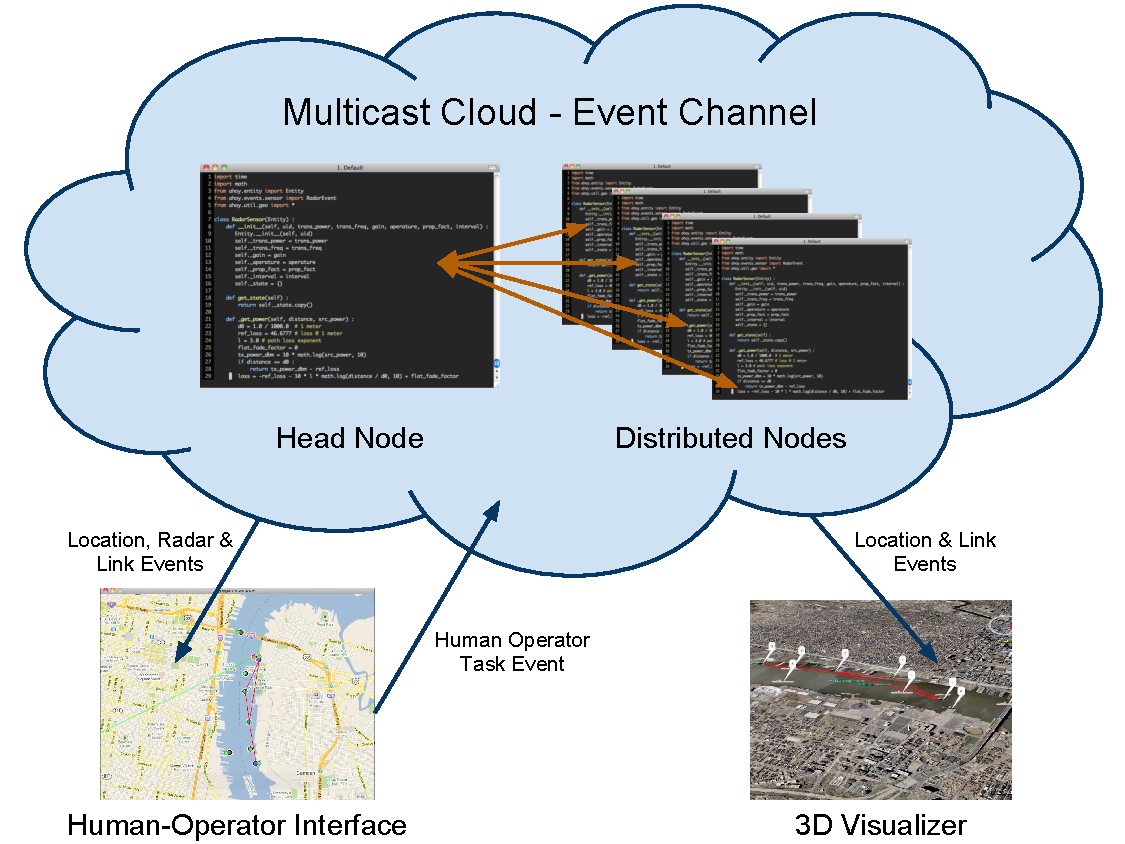
\includegraphics[scale=.48]{demo.pdf}
    \end{center}
}

%% End backup slides
\backupend

\end{document}
